% options:
% thesis=B bachelor's thesis
% thesis=M master's thesis
% czech thesis in Czech language
% english thesis in English language
% hidelinks remove colour boxes around hyperlinks

\documentclass[thesis=M,english]{FITthesis}[2012/10/20]

% \usepackage[utf8]{inputenc} % LaTeX source encoded as UTF-8
% \usepackage[latin2]{inputenc} % LaTeX source encoded as ISO-8859-2
% \usepackage[cp1250]{inputenc} % LaTeX source encoded as Windows-1250

\usepackage{graphicx} %graphics files inclusion
% \usepackage{subfig} %subfigures
% \usepackage{amsmath} %advanced maths
% \usepackage{amssymb} %additional math symbols

\usepackage{dirtree} %directory tree visualisation

\usepackage{listings}

% % list of acronyms
% \usepackage[acronym,nonumberlist,toc,numberedsection=autolabel]{glossaries}
% \iflanguage{czech}{\renewcommand*{\acronymname}{Seznam pou{\v z}it{\' y}ch zkratek}}{}
% \makeglossaries

\usepackage{color}
\definecolor{lightgray}{rgb}{.9,.9,.9}
\definecolor{darkgray}{rgb}{.4,.4,.4}
\definecolor{purple}{rgb}{0.65, 0.12, 0.82}
\lstdefinelanguage{JavaScript}{
  keywords={break, case, catch, continue, debugger, default, delete, do, else, false, finally, for, function, if, in, instanceof, new, null, return, switch, this, throw, true, try, typeof, var, void, while, with},
  morecomment=[l]{//},
  morecomment=[s]{/*}{*/},
  morestring=[b]',
  morestring=[b]",
  ndkeywords={class, export, boolean, throw, implements, import, this},
  keywordstyle=\color{blue}\bfseries,
  ndkeywordstyle=\color{darkgray}\bfseries,
  identifierstyle=\color{black},
  commentstyle=\color{purple}\ttfamily,
  stringstyle=\color{red}\ttfamily,
  sensitive=true
}

\lstset{
   language=JavaScript,
   backgroundcolor=\color{lightgray},
   extendedchars=true,
   basicstyle=\footnotesize\ttfamily,
   showstringspaces=false,
   showspaces=false,
   numbers=left,
   numberstyle=\footnotesize,
   numbersep=9pt,
   tabsize=2,
   breaklines=true,
   showtabs=false,
   captionpos=b
}

% % % % % % % % % % % % % % % % % % % % % % % % % % % % % % 
% EDIT THIS
% % % % % % % % % % % % % % % % % % % % % % % % % % % % % % 

\department{Department of Software Engineering}
\title{GPS pinned messaging application}
\authorGN{Daria} %author's given name/names
\authorFN{Mikhailova} %author's surname
\author{Mikhailova Daria} %author's name without academic degrees
\authorWithDegrees{Mikhailova Daria \& Bc.} %author's name with academic degrees
\supervisor{Jan Vaclavik}
\acknowledgements{THANKS}
\abstractEN{Summarize the contents and contribution of your work in a few sentences in English language.}
\abstractCS{V n{\v e}kolika v{\v e}t{\' a}ch shr{\v n}te obsah a p{\v r}{\' i}nos t{\' e}to pr{\' a}ce v {\v c}esk{\' e}m jazyce.}
\placeForDeclarationOfAuthenticity{Prague}
\keywordsCS{Replace with comma-separated list of keywords in Czech.}
\keywordsEN{Replace with comma-separated list of keywords in English.}
\declarationOfAuthenticityOption{1} %select as appropriate, according to the desired license (integer 1-6)


\begin{document}

% \newacronym{CVUT}{{\v C}VUT}{{\v C}esk{\' e} vysok{\' e} u{\v c}en{\' i} technick{\' e} v Praze}
% \newacronym{FIT}{FIT}{Fakulta informa{\v c}n{\' i}ch technologi{\' i}}

\setsecnumdepth{part}
\chapter{Introduction}



\setsecnumdepth{all}
\chapter{Requirements}
\section{Messaging application}

Usual messaging applications require the communicating parties to identify themselves with each other, either using their phone numbers or emails. The GPS pinned application does not require any details from the other party in order to communicate. The idea is very simple. Imagine you are travelling and you just moved in a hotel. You do not know anyone in the city and would like to have a company for the sightseeing. In this case you just leave a message right in your room and everyone in the hotel would see it, since they would be within a short reach o your GPS location. Anyone could answer your message and probably very quickly you will manage to find yourself a company for the walk in the city.

The main goal is to create a messaging application which will allow users to pin messages to GPS location. There will be two types of messages. Firstly users will post simple text messages with an option of attaching a picture. Secondly users are able to post a 3D object. Both types of messages are commentable. Each posted message can have a validity from 1 hour up to infinity. Users are only able to read a message once they arrive at its GPS location. Once the user reads the message he can later comment on it even though he/she is not within the message's GPS reach. Read messages are added to user's list of messages and he can get back later to them. The user will be notified in case someone commented on his message or any of the messages he commented on received a new comment.

\section{Functional requirements}

\begin{enumerate}
\item{Registration}

User can register using their email and password or sign in through Facebook.

\item{Authentication}

Users will be authenticated through tokens using OAuth protocol. Authentication through Facebook with OpenID protocol will also be available.

\item{Leave a message}

The user is able to leave a message pinned to his/her GPS location. There is an option of adding an image to the message.

\item{Leaving a 3D object}

The user is able to leave a 3D object pinned to his/her GPS location. The user can choose a 3D object from the gallery of object or upload their own object following the instructions on the web.

\item{Read a message}

The user is able to read a message only once he/she is close to its GPS location.

\item{Comment message}

The user is able to comment any message he has stumbled upon.

\item{User gets notifications about messages}

When the user is in the certain radius of the message he will get a notification on his mobile about it

\item{View statistics}

Users can view statistics of their messages, how often it has been read, how many replies.
Admin users can also view general statistics, which areas are popular, which messages in which areas get replies and which do not. Possible analysis of message content, what users like, what they reply on.

\item{View and change user details}

The user has a choice of either showing details about himself or not. The only compulsory public detail is username.

\end{enumerate}

\section{Non functional requirements}

\begin{enumerate}

\item{Performance} 

There must be short response time for server requests.

\item{Resources} 

The application should not consume too much battery power in both active and idle modes.

\item{Usability}

User friendly interface in IOS style so the users know how to use the application intuitively.

\item{Recoverability}

should be able to recover fast in case of server crash or any other fails

\item{Data Integrity}

the messaging and other data has to be consistent in any situation.

\item{Reliability}

the application should be able to take care of spam.

\item{Documentation}

extensive and detailed documentation must be provided

\item{Extensibility}

the application should be created using technologies that it would be easy to extend and create new features in the future

\item{Scalability}

the application needs to be able to cope with a growing amount of requests 
\end{enumerate}

\chapter{Analysis and design}
\section{Technology used}
\subsection{Node.js}

Node.js is a runtime environment, it is open source and cross-platform, most of it is written in Javascript. Node.js REST API web server will be implemented to serve as a backend for both mobile and web applications.

Node.js uses non blocking event-driven I/O to remain flexible and lightweight when faced with intensive real-time application with high data transfer demands.\cite{why-node} The non blocking part means that commands are executed in parallel and they use callbacks to signal completion. For instance in a blocking language such as PHP, the command executes only after previous command has finished running.\cite{node-benefits} Node should not be used for heavy computations, since it will eliminate all of its benefits. Node manipulates with one thread. Therefore resource consuming computations can clog the thread and prevent other requests from being processed. It is best used for creating fast, scalable network applications, since its biggest advantage is its ability to handle a massive number of simultaneous connections. Another massive advantage of Node.js is built in support for package management using NPM tool. NPM provides the developer with a set of reusable components which are easily installed and used in the project. It is one of the largest set of open source libraries.\cite{nodejs}

The way Node.js works is demonstrated on figure \ref{fig:nodejs}. The whole action of Node.js happens in the Event loop. Event loop is a set of events defined in your application which node is waiting for to be fired. Once an application sends a request, an event is fired and is placed in the event queue. Event loop picks up the event  and processes it. In the case that the event is blocking such (e.g. image reading) it passes its processing to one of its worker threads from its own worker thread pool. When the worker is finished processing the event, it returns the response using a callback which was passed to it with the task. The result is passed to the application through Node.js bindings \cite{node-benefits}

\begin{figure}[!ht]
	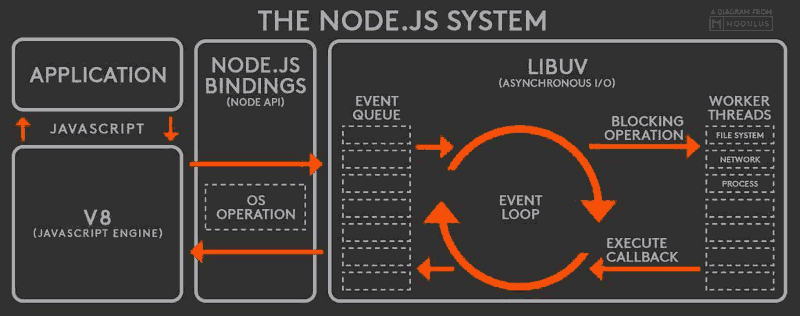
\includegraphics[width=1\textwidth]{assets/nodejs_system.png}}
	\caption{Node.js system}	
	\label{fig:nodejs}
\end{figure}

The main advantages of running a node.js server:

\begin{itemize}
\item{} Node.js server can asynchronously process incoming requests. Therefore the response rate is faster. 

\item{} Node.js is event-driven, and uses non blocking I/O by utilising callbacks, event loop and event queue. This means that we use browser style concurrency model on the web server.

\item{} Since it is javascript we are able to take advantage of the V8 Javascript Engine. V8 Javascript Engine compiles Js code into native machine code which brings better performance comparing to usual techniques such as interpreting.

\item{} Node js is well suited for real time application that run across various devices. It is perfect for fast delivering of data to many requestors at the same time.
\end{itemize}



Figure \ref{fig:nodejsVsTraditional} shows a comparison of request processing on a node server and a traditional web server (e.g. web server Apache). On a traditional web server where for each request a new connection thread is created from a limited thread pool or the server waits for any of the working threads to finish so it can delegate the request to them. Many threads use a lot of RAM and the system eventually slows down or even crashes in case of a lot of requests.
What Node.js does differently is it operates on a single-thread using non blocking I/O calls, which allows it to support a lot of simultaneous connections.
Assume that each request-thread will demand 2MB of memory. Let's also assume that the server is running on an 8GB of RAM. This leaves us with a conclusion that when using a traditional web server it is capable of processing about 4000 simultaneous requests. Node.js in contrary is theoretically able to process over 1M simultaneous requests due to its scalability. \cite{why-node}

\begin{figure}[!ht]
	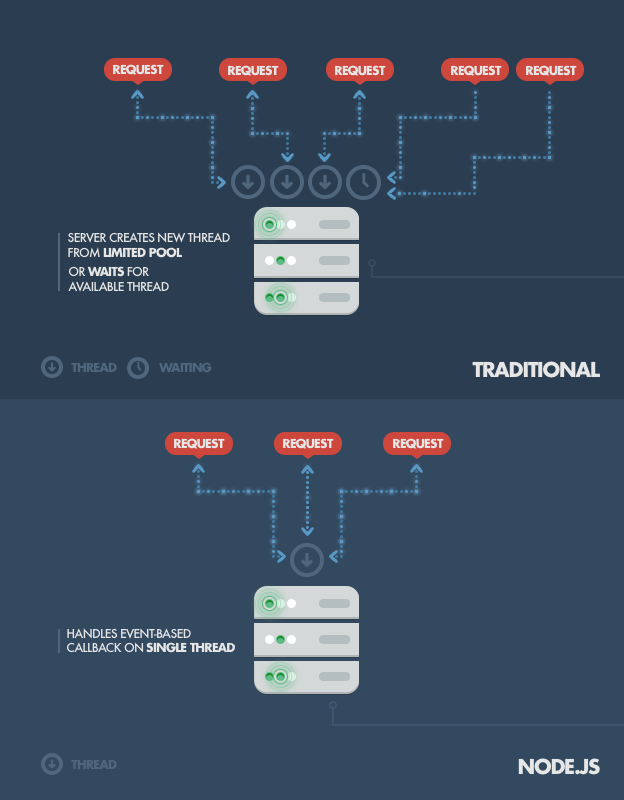
\includegraphics[width=1\textwidth]{assets/nodejsVsTraditional.png}}
	\caption{Node.js server processing compared with traditional web server processing of requests}	
	\label{fig:nodejsVsTraditional}
\end{figure}


\newpage
\subsection{React}
React is a very flexible view layer written in javascript. 
%http://developer.telerik.com/featured/introduction-to-the-react-javascript-framework/
It has several advantages the main one being the way it is organised. It breaks down the application into components and makes it very easy to make changes without affecting other code. The components, each of them representing a single view (e.g. a button, form), can be reused for other applications since each component represents an independent part of the programme.

It uses a declarative programming style. Declarative programming means we tell the machine what we want to see as the result and let it figure out how it should be done.

React's way of creating application might not seem correct to many developers since it embeds css in javascript, which has been considered a bad practice throughout the past decade. Mixing markup with logic is what we have been always trying to avoid. However there are quite a few issues with CSS which React JS, due to its approach, solves without any hacks. For instance no need to worry about dependencies, dead code elimination, minification, isolations, etc. Moreover this approach allows us to create independent and easy to read component which can be changed at any time without worrying about affecting the rest of the application.

One of the biggest advantages is the virtual DOM. React does not re-render the whole DOM every time you make a change. React creates a diff between the existing DOM and you changes and applies the patch to the existing DOM, changing only a part of it and saving loads of time.

Server rendering is another very important point. Server rendering allows to render the whole page on the server side (e.g. Node.js), which is faster and SEO-friendly. Both virtual DOM and server side rendering make React's performance very high.

Furthermore React has good descriptive warnings which make the debugging process easy. Its declarative approach makes the code predictable and easier to understand. Therefore the learning curve is flat and developers start making changes with confidence faster. 

React relies on unidirectional data flow. The data, called props in React, are passed from parent to child. When the props change the component is re-rendered in order to keep up to date with the application data changes. Also every component has its own private data called state.

\subsection{ReactNative}

\subsubsection{Why not use Native?}
%https://code.facebook.com/posts/1014532261909640/react-native-bringing-modern-web-techniques-to-mobile/
The native mobile development is difficult and cumbersome. Firstly it is difficult to place different components of your app on the screen since you often need to compute exact positions of all of your views. Moreover every time the developer makes a change in the app they need to recompile the whole application, even if it is the smallest change, such as enlarging fontSize. This takes a lot of time from the development process and therefore slows down the whole development cycle. In case the developer wants to create a multi platform application, let's say for iOS, Android and Windows, they need to write the same application three times in three completely different languages. Apart from the need to learn specific platform implementation and principles, which are usually not reusable for other platforms, the developer also has to think about memory management, thread concurrency and deployment process. All these issues are important and bring a necessary overhead when developing native applications

Even though development of native applications is a lengthy and difficult process, there are reasons why it is worth it. One of the main reasons why developers go and make native apps is the access to mobile native functions which allow to create a better-feeling experience, such as UI components - date pickers, sliders, etc. This main feature of native development is reproduced in ReactNative as you can read further.

\subsubsection{Why ReactNative?}

The GPS pinned mobile application will be implemented using React Native. It is the first JS framework which works with mobile's native functions directly, which is it's huge advantage.

React Native runs the code using an interpreter and provides a native bridge to construct and fully interact with platform native elements. In comparison to React which renders divs and spans in the browser React Native renders native higher-level platform-specific components inside of an embedded instance of JavaScriptCore inside the application. It also allows to use CSS Flexbox which creates a better User Experience and an easier placement of the elements with no need for computing their position.

Furthermore working with React is faster than with other platform native languages, since you do not have to recompile the whole app any time you make the tiniest change, you just refresh the application and view your changes straight away. Its very handy since it saves a lot of development time. React Native also provides us with the ability of parallelising the work, which increases the speed of the application.

This framework introduces a totally new approach for developing mobile apps and enforces a new principle: 'Learn once, write anywhere'. Facebook provides implementations and support both IOS and Android versions. Since React Native is a very recent framework it does not fully support native features for both systems. At the moment Facebook has more components and APIs ready for use with IOS than with Android. Android, on the other hand has a lot of open source components which are easily accessible.

ReactNative can be used alongside with the native code. In order to use native code functions the developer has to create a bridge between ReactNative and native and export the functions they want to use in javascript.

The last but not the least, ReactNative uses React, view framework described earlier.

\subsection{Objective C}

\subsection{MongoDb}
MongoDb is a non relational database which stores its data in files. If well designed it provides a very fast way of retrieving data. Among the main advantages over usual RDBMS belong:

\begin{enumerate}
\item{Easy structure.} You do not need to create a lot of difficult relations, foreign keys and relation tables in your schema, since there is no schema. It is a document base database, which holds collections of documents.

\item{No complex joins.} When retrieving data you simply ask for a certain document and get all the needed information straight away. It takes just one request to the database to get your data.

\item{Flexible.} It usually happens that some entities populate certain fields and some do not and then the developer ends up with a lot of NULL value fields. Also adding/removing a new field to/from the RDBMS gets very complex, depending on the relations and the data which the database is already filled in with. Mongodb provides incredible flexibility here, since you can just add fields in some documents and do not add them in others. Doing so you eliminate null value fields and also get rid of the problem of adding/removing the field without breaking the whole structure.

\item{Easy conversion.} The data in Mongodb is stored in json format, therefore once retrieved it is ready to use, with no need of conversion and mapping between formats and structures.

\item{Query ability.} MongoDb uses its own query language which is similar to SQL, and therefore easy to learn to those who are familiar with SQL.
\end{enumerate}

\subsection{Augmented Reality}

One of the functionalities of a GPS pinned messaging application is the ability 
One of the options this mobile application provides is leaving 3D objects pinned to GPS. In order to implement this I used technology used Augmented Reality.

Augmented reality is the real world enhanced by the virtual reality. Virtual reality objects are placed in the real world settings and can be viewed with the help of various devices: mobiles, tablets, smart glasses etc. 

There are several different types of Augmented reality:
\begin{itemize}
	\item{Marker based AR} \cite{ar-research}
	\item{Markerless AR}
	\item{POI}
	\item{Location based AR}
\end{itemize}

\section{Database}
lala

\section{Server}
lalla

\section{Augmented Reality}
\label{section:ar}

After conducting a thorough research concerning various Augmented reality implementations, techniques and frameworks I limited my options to three choices. My goal is to be able to place a 3D object at a given GPS location. Therefore I was looking for a location aware solution. Below are listed different AR solutions I was considering.

\begin{itemize}
	\item{Open source Augmented Reality SDK}
	
	There are a few open source AR SDKs with IOS support, implemented in Objective C. The one which seemed to be the most relevant can be found at  https://github.com/promet/PRAugmentedReality. This is neat small framework which supports even the older iPhones. It supports a type of AR called POI or Points Of Interest. It is not that well documented but has a video tutorial on how to get started with the framework. The lack of documentation is compensated with well commented code and a sample application.
	
	Advantages:
	\begin{itemize}
		\item{Support for Points of Interset}
	\end{itemize}
	
	Disadvantages:
	\begin{itemize}
		\item{No support for 3D object which means the user would have to implement 3D object rendering himself}
		\item{Implemented in Objective C, which is not the most developer friendly language}
		\item{The last update of the framework was performed 2 years ago. This basically means the framework is not supported anymore. There is no community and in case of problems or bugs the developer has to deal with everything himself. There is an option of communicating with the author, but he didn't respond to my email inquiring about the possible support of 3D images, so I would not rely on that.}
	\end{itemize}

	Conclusion:
	This option does not seem to be suitable as it is requires a deep understanding of Objective C in order to implement rendering and fix possible problems which might arise during development.

	\item{Unity 3D - Kudan AR plugin}
	
	Advantages:
	\begin{itemize}
		\item{SLAM} - Simultaneous localization and mapping
		\item{c}
		
	\end{itemize}
	
	Disadvantages:
	\begin{itemize}
		\item{a}
		\item{b}
	\end{itemize}	
	\item{Wikitude AR}
	Advantages:
	\begin{itemize}
		\item{Javascript API}
		\item{Big community}
		\item{Support}				
	\end{itemize}
	
	Disadvantages:
	\begin{itemize}
		\item{Trial version} - the only free version, however with full support of all SDK's features, is trial. There is a watermark on the camera screen when using AR.
	\end{itemize}		
\end{itemize}


After careful consideration I decided to choose the 3d option - Wikitude AR SDK with trial version. It seems to be the best solution.

\subsection{Server design}
lala

\subsection{Api design}
lala

\section{Mobile application}
lalal
\subsection{Application design}
My mobile application is built with React Native which is a view framework. It is a frontend The MVC concept, however very familiar to me didn't seem at the right place. 

\subsubsection{Redux}
Redux is a predictable state container for Javascript application. It is a small library which helps control and structure application's state hierarchy.

The main concern in javascript application is taking care of the state of application. 

Redux was created inspired by Flux which is a way Facebook creates their applications.
Flux
Why is Redux better?

\subsubsection{Data Flow}
Redux's biggest advantage it's the way it handles the data flow. Redux has unidirectional data flow, which provides the developer with a clear and easy to debug application.

The structure of the application using redux is shown on \ref{fig:redux}. Each part of the scheme plays vital role.
\begin{itemize}
\item{Presentational and Container Components}

Presentational components are components which do not hold any logic inside themselves. Everything they need for functioning they receive passed in their props from the Container Components. In the case presentational component needs to fire an event it uses callbacks which are passed to it in props. There is no logic in Presentational Components.


Container Components are the once who dispatch events when presentational components receive user interaction. They also take care of navigation. Sometimes they referred to as smart components and presentational components as dumb components.

\item{Action makers}

Action makers are the ones who return actual action objects for the actions dispatched in Container Components.

\item{Store}

Store holds the application state. The application state changes with different actions and throughout the whole run of the application it is held by the store. Application state can be defined as a set of objects, collections of objects, cached data from the server, there could be booleans, integer or string values which are requested by the application. For instance the state can hold an authentication cookies value f the user has been successfully logged in the system.

\item{Reducers}

Reducers are pure functions. Pure functions are functions which do not modify their arguments. Reducers accept as argument the current state of the application and an action which was dispatched. They return a new state of the application, by returning a completely new object, could be the clone of the current state but can never be a modified current state. This is due to the reasons that i ll explain later (components subscribed to props). Reducers are basically state machines which tell which state follows after the state you are in if you do the given action.

\end{itemize}

\begin{figure}[!ht]
	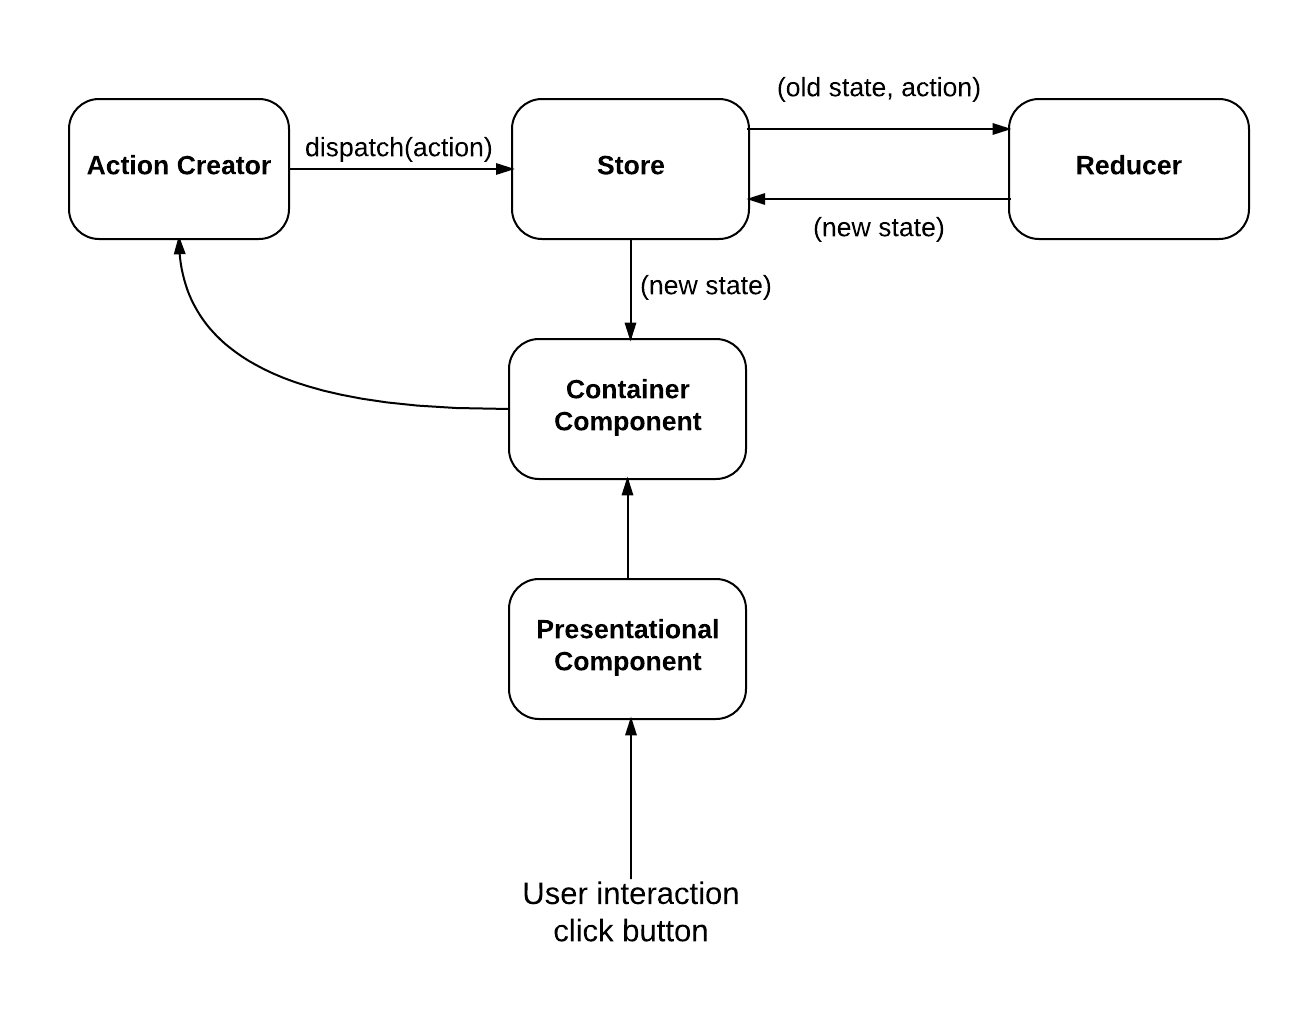
\includegraphics[width=1\textwidth]{assets/redux.png}}
	\caption{Redux structure. Unidirectional dataflow.}	
	\label{fig:redux}
\end{figure}



Action creation rules
https://github.com/acdlite/flux-standard-action

Reducer composition

\section{Web application}
lala

\subsection{Application design}
lala

\chapter{Realisation}

\section{Augmented Reality}
As I have previously stated in chapter Analysis and design section \nameref{section:ar} I chose Wikitude SDK for implementation of Augmented Reality in my application. 

Wikitude SDK has a plugin for IOS development with Javascript API which I decided to use. There is no direct support for React Native, but the plugin provides a developer with Wikitude framework and there is a set of instructions how to integrate AR in the native iOS application on their website (for reference see official setup guide \url{http://www.wikitude.com/developer/documentation/ios}. 

\subsection{Connecting React Native and Objective C}
React Native is a set of javascript functions wrapped around native code. Therefore you can make your application communicate with the native code using Native Modules or Native UI Components. This is particularly useful when you want to implement part of you application's functionality natively.  

There are two macros which are used for this case:

\begin{itemize}
\item  \verb|RCT_MODULE_EXPORT()| 
This macro says that the given class is exported to React Native and can be referenced by its name. It is considered to be good programming style to separate your files into header (\verb|.h| extension) and implementation files (\verb|.m| extension). For an example of exporting a module see the following classes: \verb|ExampleManager.h|, \verb|ExampleManager.m| and \verb|Component.js|.


\begin{lstlisting}[language=C]
// ExampleManager.h
#import "RCTViewManager.h"

@interface ExampleManager : RCTViewManager
@end

\end{lstlisting}

\begin{lstlisting}[language=C]
// ExampleManager.m
#import <YourCustomView.h>

#import "RCTViewManager.h"
#import "ExampleManager.h"

@implementation ExampleManager

RCT_EXPORT_MODULE()

- (UIView *)view
{
  return [[YourCustomView alloc] init];
}

@end
\end{lstlisting}

\begin{lstlisting}[language=javascript]
// Component.js
import React, { requireNativeComponent } from 'react-native';

var Example = requireNativeComponent('Example', Component);

class Component extends React.Component {
  render() {
    return <Example />;
  }
}

module.exports = Component;
\end{lstlisting}
  
  \verb|ExampleManager.h| is a header file and it solely defines interface and possible attributes or parameters for the main class. For our purposes it extends RCTViewManager who takes care of views in React Native, hence the suffix RCT.
  
  \verb|ExampleManager.m| implements \verb|view| function which returns \verb|UIView*| on line 11. This function is called by default on any class representing a view in Objective C, when it is mounted in the view hierarchy.
  
  \verb|Component.js| is the actual component we use in our React Native application. In order to use Native UI Component which we defined in  \verb|ExampleManager.h| and \verb|ExampleManager.m| we add an import as stated on line 2 and require native component on line 4. After that the native view is ready to use as a simple react component as you can see on line 8.
  
\item  \verb|RCT_METHOD_EXPORT(*method*)|

\end{itemize}

\subsection{Integration of Wikitude and RN}
To start using Wikitude SDK we first need to add it to our XCode project and create a ViewController as described in the official setup guide at \url{http://www.wikitude.com/developer/documentation/ios}. There is also a sample project available at \url{https://github.com/Wikitude/wikitude-sdk-basic-projects} which shows an example of ViewController implementation. For my purposes I had to modify the sample implementation. The complete implementation for integration of Wikitude and React Native is found in Appendix: \nameref{apendix:integration}

\setsecnumdepth{part}
\chapter{Conclusion}


\bibliographystyle{iso690}
\bibliography{bibliography/bibliography}

\setsecnumdepth{all}
\appendix

\chapter{Acronyms}
% \printglossaries
\begin{description}
	\item[GUI] Graphical user interface
	\item[XML] Extensible markup language
\end{description}

\chapter{Integration of Wikitude and React Native}
\label{apendix:integration}
In order to integrate Wikitude and React Native I implemented the following files:
\begin{itemize}
\item \verb|ViewController.h| 
\item \verb|ViewController.m| - starting point for the Wikitude
\item \verb|ARViewManager.h|
\item \verb|ARViewManager.m| - exported view component for React Native
\end{itemize}

\begin{lstlisting}[language=C]
//  ViewController.h

#import <UIKit/UIKit.h>

@interface ViewController : UIViewController

-(UIView*)start;

@end

\end{lstlisting}

\begin{lstlisting}[language=C]
//  ViewController.m

#import "ViewController.h"
#import <WikitudeSDK/WikitudeSDK.h>
/* Wikitude SDK debugging */
#import <WikitudeSDK/WTArchitectViewDebugDelegate.h>

@interface ViewController () <WTArchitectViewDelegate, WTArchitectViewDebugDelegate>

/* Add a strong property to the main Wikitude SDK component */
@property (nonatomic, strong) WTArchitectView *architectView;

/* And keep a weak property to the navigation object which represents the loading status of your Architect World */
@property (nonatomic, weak) WTNavigation *architectWorldNavigation;

@end


@implementation ViewController

- (void)dealloc
{
  [[NSNotificationCenter defaultCenter] removeObserver:self];
}

- (UIView*)start {
  NSError *deviceSupportError = nil;

  if ( [WTArchitectView isDeviceSupportedForRequiredFeatures:WTFeature_Geo error:&deviceSupportError] ) {
    
    /* Standard WTArchitectView object creation and initial configuration */
    self.architectView = [[WTArchitectView alloc] initWithFrame:CGRectZero motionManager:nil];
    self.architectView.delegate = self;
    self.architectView.debugDelegate = self;
    
    /* Use the -setLicenseKey method to unlock all Wikitude SDK features that you bought with your license. */
    [self.architectView setLicenseKey:@"licenceKey"];
    
    /* The Architect World can be loaded independently from the WTArchitectView rendering.
     
     NOTE: The architectWorldNavigation property is assigned at this point. The navigation object is valid until another Architect World is loaded.
     */
    
    NSURL *baseURL = [NSURL URLWithString:(@"http://url-to-your/architect-world/index.html")];
    self.architectWorldNavigation = [self.architectView loadArchitectWorldFromURL:baseURL withRequiredFeatures:WTFeature_Geo];
    
    /* Because the WTArchitectView does some OpenGL rendering, frame updates have to be suspended and resumend when the application changes it's active state.
     Here, UIApplication notifications are used to respond to the active state changes.
     
     NOTE: Since the application will resign active even when an UIAlert is shown, some special handling is implemented in the UIApplicationDidBecomeActiveNotification.
     */
    [[NSNotificationCenter defaultCenter] addObserverForName:UIApplicationDidBecomeActiveNotification object:nil queue:[NSOperationQueue mainQueue] usingBlock:^(NSNotification *note) {
      
      /* When the application starts for the first time, several UIAlert's might be shown to ask the user for camera and/or GPS access.
       Because the WTArchitectView is paused when the application resigns active (See line 86), also Architect JavaScript evaluation is interrupted.
       To resume properly from the inactive state, the Architect World has to be reloaded if and only if an active Architect World load request was active at the time the application resigned active.
       This loading state/interruption can be detected using the navigation object that was returned from the -loadArchitectWorldFromURL:withRequiredFeatures method.
       */
      if (self.architectWorldNavigation.wasInterrupted) {
        [self.architectView reloadArchitectWorld];
      }
      
      /* Standard WTArchitectView rendering resuming after the application becomes active again */
      [self startWikitudeSDKRendering];
    }];
    [[NSNotificationCenter defaultCenter] addObserverForName:UIApplicationWillResignActiveNotification object:nil queue:[NSOperationQueue mainQueue] usingBlock:^(NSNotification *note) {
      
      /* Standard WTArchitectView rendering suspension when the application resignes active */
      [self stopWikitudeSDKRendering];
    }];
    
    /* Standard subview handling using Autolayout */
    [self.view addSubview:self.architectView];
    self.architectView.translatesAutoresizingMaskIntoConstraints = NO;
    
    NSDictionary *views = NSDictionaryOfVariableBindings(_architectView);
    [self.view addConstraints: [NSLayoutConstraint constraintsWithVisualFormat:@"|[_architectView]|" options:0 metrics:nil views:views] ];
    [self.view addConstraints: [NSLayoutConstraint constraintsWithVisualFormat:@"V:|[_architectView]|" options:0 metrics:nil views:views] ];
    return self.view;
  }
  else {
    NSLog(@"This device is not supported. Show either an alert or use this class method even before presenting the view controller that manages the WTArchitectView. Error: %@", [deviceSupportError localizedDescription]);
    return nil;
  }
}

#pragma mark - View Lifecycle
- (void)viewWillAppear:(BOOL)animated {
  NSLog(@"%s", "will appear");
  [super viewWillAppear:animated];
  
  /* WTArchitectView rendering is started once the view controllers view will appear */
  [self startWikitudeSDKRendering];
}

- (void)viewDidDisappear:(BOOL)animated {
  NSLog(@"%s", "will dissappear");
  [super viewDidDisappear:animated];
  
  /* WTArchitectView rendering is stopped once the view controllers view did disappear */
  [self stopWikitudeSDKRendering];
}

- (void)didReceiveMemoryWarning {
  [super didReceiveMemoryWarning];
  // Dispose of any resources that can be recreated.
}

#pragma mark - View Rotation
- (BOOL)shouldAutorotate {
  
  return YES;
}

- (NSUInteger)supportedInterfaceOrientations {
  
  return UIInterfaceOrientationMaskAll;
}

- (void)willRotateToInterfaceOrientation:(UIInterfaceOrientation)toInterfaceOrientation duration:(NSTimeInterval)duration {
  
  /* When the device orientation changes, specify if the WTArchitectView object should rotate as well */
  [self.architectView setShouldRotate:YES toInterfaceOrientation:toInterfaceOrientation];
}

#pragma mark - Private Methods

/* Convenience methods to manage WTArchitectView rendering. */
- (void)startWikitudeSDKRendering{
  
  /* To check if the WTArchitectView is currently rendering, the isRunning property can be used */
  if ( ![self.architectView isRunning] ) {
    NSLog(@"architect running. started");
    /* To start WTArchitectView rendering and control the startup phase, the -start:completion method can be used */
    [self.architectView start:^(WTStartupConfiguration *configuration) {
      
      /* Use the configuration object to take control about the WTArchitectView startup phase */
      /* You can e.g. start with an active front camera instead of the default back camera */
      
    } completion:^(BOOL isRunning, NSError *error) {
      
      /* The completion block is called right after the internal start method returns.
       
       NOTE: In case some requirements are not given, the WTArchitectView might not be started and returns NO for isRunning.
       To determine what caused the problem, the localized error description can be used.
       */
      if ( !isRunning ) {
        NSLog(@"WTArchitectView could not be started. Reason: %@", [error localizedDescription]);
      }
    }];
  }
}

- (void)stopWikitudeSDKRendering {
  
  /* The stop method is blocking until the rendering and camera access is stopped */
  if ( [self.architectView isRunning] ) {
    [self.architectView stop];
  }
}

/* The WTArchitectView provides two delegates to interact with. */
#pragma mark - Delegation

/* The standard delegate can be used to get information about:
 * The Architect World loading progress
 * architectsdk:// protocol invocations using document.location inside JavaScript
 * Managing view capturing
 * Customizing view controller presentation that is triggered from the WTArchitectView
 */
#pragma mark WTArchitectViewDelegate
- (void)architectView:(WTArchitectView *)architectView didFinishLoadArchitectWorldNavigation:(WTNavigation *)navigation {
  /* Architect World did finish loading */
}

- (void)architectView:(WTArchitectView *)architectView didFailToLoadArchitectWorldNavigation:(WTNavigation *)navigation withError:(NSError *)error {
  
  NSLog(@"Architect World from URL '%@' could not be loaded. Reason: %@", navigation.originalURL, [error localizedDescription]);
}

/* The debug delegate can be used to respond to internal issues, e.g. the user declined camera or GPS access.
 
 NOTE: The debug delegate method -architectView:didEncounterInternalWarning is currently not used.
 */
#pragma mark WTArchitectViewDebugDelegate
- (void)architectView:(WTArchitectView *)architectView didEncounterInternalWarning:(WTWarning *)warning {
  
  /* Intentionally Left Blank */
}

- (void)architectView:(WTArchitectView *)architectView didEncounterInternalError:(NSError *)error {
  
  NSLog(@"WTArchitectView encountered an internal error '%@'", [error localizedDescription]);
}

@end
\end{lstlisting}

\clearpage
\begin{lstlisting}[language=C]
//  ARViewManager.h

#import "RCTViewManager.h"

@interface ARViewManager : RCTViewManager

@end

\end{lstlisting}

\begin{lstlisting}[language=C]
//  ARViewManager.m

#import "ARViewManager.h"
#import "ViewController.h"

@implementation ARViewManager

RCT_EXPORT_MODULE()

- (UIView *)view
{
    ViewController* controller = [[ViewController alloc] init];
    return [controller start];
}

@end
\end{lstlisting}

\chapter{Contents of enclosed CD}

%change appropriately

\begin{figure}
%	\dirtree{%
%		.1 readme.txt\DTcomment{the file with CD contents description}.
%		.1 exe\DTcomment{the directory with executables}.
%		.1 src\DTcomment{the directory of source codes}.
%		.2 wbdcm\DTcomment{implementation sources}.
%		.2 thesis\DTcomment{the directory of \LaTeX{} source codes of the thesis}.
%		.1 text\DTcomment{the thesis text directory}.
%		.2 thesis.pdf\DTcomment{the thesis text in PDF format}.
%		.2 thesis.ps\DTcomment{the thesis text in PS format}.
%	}
\end{figure}

\end{document}
